\section{LabVIEW als Programmiersprache}
	\label{sec:labview}
	
LabVIEW ist ein grafisches Programmiersystem von National Instruments. Das Akronym steht für "`Laboratory Virtual Instrumentation Engineering Workbench"'.

Die Programmierung erfolgt in der graphischen Programmiersprache "`G"'.  LabVIEW-Programme werden als Virtuelle Instrumente (VIs) bezeichnet. \cite{ni-tuto}
%\cite{wiki-lv}

Sie bestehen aus drei Komponenten: 
\begin{description}
	\item[Frontpanel] Das User-Interface, über welches der Anwender mit dem VI interagiert.
	\item[Blockdiagramm] Stellt den Programmcode des VIs dar.
	\item[Anschluss] Dient zur Anbindung an weitere VIs. Bestimmt Übergabe und Rückgabe Werte. 
\end{description}

In LabVIEW liegt die Ausführung von VIs dem Datenflussmodell zugrunde. Ein Blockdiagrammknoten (Bsp. Addition) wird ausgeführt, sobald all seine Eingänge belegt sind. Ist die Ausführung eines Knotens abgeschlossen, werden die Daten an die Ausgabeanschlüsse übergeben und die Ausgabedaten dann an den nächsten Knoten im Datenflussdiagramm weitergeleitet. \cite{LVT}
Die unter LabVIEW erstellten Blockdiagramme werden von einem grafischen Compiler in optimierten Maschinencode übersetzt. Dadurch ist die Performance vergleichbar mit der anderer Hochsprachen wie C oder Pascal. \cite{ni-compiler}

Abbildung \ref{fig:demo01} zeigt eine kleine Demonstration. Es wird aus den Eingängen A und B ein Ausgang C berechnet. Die Formel wird im Blockdiagramm abgebildet. Sie lautet:
\[ C = \frac{A+B}{4}^{2} \]
Des Weiteren findet die Berechnung in einer While-Schleife statt. Die Abbruchbedingung ist die Betätigung der Stopp-Schaltfläche. 

	\begin{figure}%[h!]
	\centering
		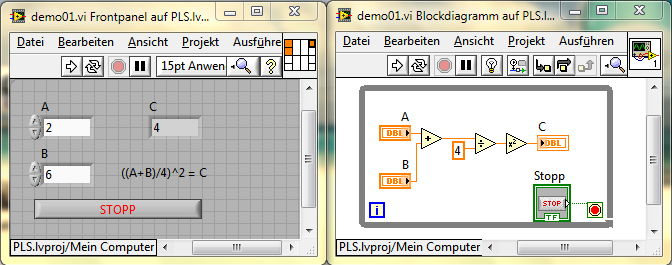
\includegraphics[width=0.7\textwidth]{Pics/demo01.png}
	\caption{VI Demonstration: Links Frontpanel, Rechts Blockdiagramm}
	\label{fig:demo01}
	\end{figure}

	%\subsection{Objektorientiertes Design}  %2-15
	\subsection{Entwurfsmuster - Design Pattern}
Zur Entwicklung einer umfangreichen Applikation ist es unerlässlich mit Entwurfsmustern zu arbeiten. Sie helfen nicht nur dem Entwickler den Überblick nicht zu verlieren sondern machen es auch für Außenstehende einfacher den Code zu lesen und modifizieren.

LabView bietet neun verschiedene Entwurfsmuster. Für welches man sich entscheidet hängt von folgenden Kriterien ab:
\begin{itemize}
	\item Gibt es eine feste Reihenfolge / Sequenzen von Befehlen?
	\item Muss das Programm mit einem User-Interface agieren?
	\item Ist die Datenverarbeitung intensiv? 
	\item Gibt es parallele Operationen?
\end{itemize}

Im folgenden gehe ich auf einige Entwurfsmuster ein, die für meine Problemstellung infrage kommen könnten. Das sind: der Zustandsautomat, Master/Slave-Entwurfsmuster, Ereignisbehandler für Benutzeroberfläche und das Erzeuger/Verbraucher-Entwurfsmuster. Später im XXX Kapitel, nach der Programmanalyse, werde ich auf meine Wahl des Entwurfsmuster eingehen.

\subsubsection{Zustandsautomat}%4-6
Mit jedem Zustand wird ein bestimmter Blockdiagramm Ausschnitt ausgeführt und ermittelt, zu welchem Zustand weitergesprungen wird. In einer While-Schleife wird eine Case-Struktur ausgeführt. 
%Die Case-Struktur bekommt Initialisierungs-Zustand. In jedem Case der Case-Struktur wird auf eine anderen Case oder den eigenen weiter gesprungen bis die While-Schleife ihre Abbruchbedingung erreicht hat.
	
\subsubsection{Master/Slave-Entwurfsmuster}
Bei diesem Entwurfsmuster gibt es eine Master-Schleife und mindestens eine Slave-Schleife. Die Master Schleife wird immer ausgeführt. Sie benachrichtigt Slave-Schleifen, einen bestimmten Code auszuführen. Die Slave-Schleifen werden vollständig ausgeführt und warten dann auf die nächste Benachrichtigung.

\subsubsection{Einfacher Ereignisbehandler für Benutzeroberfläche}
Dieses Entwurfsmuster wird verwendet für die Verarbeitung von Ereignissen der Benutzeroberfläche. Die Vorlage eignet sich für Dialogfelder und andere Programmoberflächen. Des Weiteren kann man benutzerdefinierte Ereignisse erzeugen und ausführen, die wie Ereignisse der Benutzeroberfläche behandelt werden.

\subsubsection{Erzeuger/Verbraucher-Entwurfsmuster} %4-10 
Hier werden zwei separate While-Schleifen unabhängig voneinander ausgeführt: Die erste Schleife erzeugt Daten, während die zweite Schleife die Daten verarbeitet. Obwohl sie parallel ausgeführt werden, werden zwischen den Schleifen über Queues Daten ausgetauscht.
Diese Vorlage bietet die Möglichkeit bei Benutzereingriffen asynchron Code auszuführen, ohne die Reaktionszeit der Benutzeroberfläche zu beeinträchtigen. 
So kann man durch die parallele Ausführung der Schleifen Leistungssteigerung des Programms erzielen. 

		
		%\paragraph{Event Handling}
		%\paragraph{Error Handling} %4-47
		
\section{Programm Analyse}
		%\subsection{Programmablaufplan} %2-18
\subsection{Ablaufdiagramm }
Mit Ablaufdiagrammen wird der Programmfluss illustriert. Mit deren Hilfe kann man eine Aufgabe in handhabbare Funktionen teilen. Abbildung \ref{fig:plan01} zeigt das Ablauf Diagramm für die Abspiel-Funktion in der Party-Licht-Steuerung. Ein Knoten repräsentiert eine Funktion.
	\begin{figure}[h!]
	\centering
		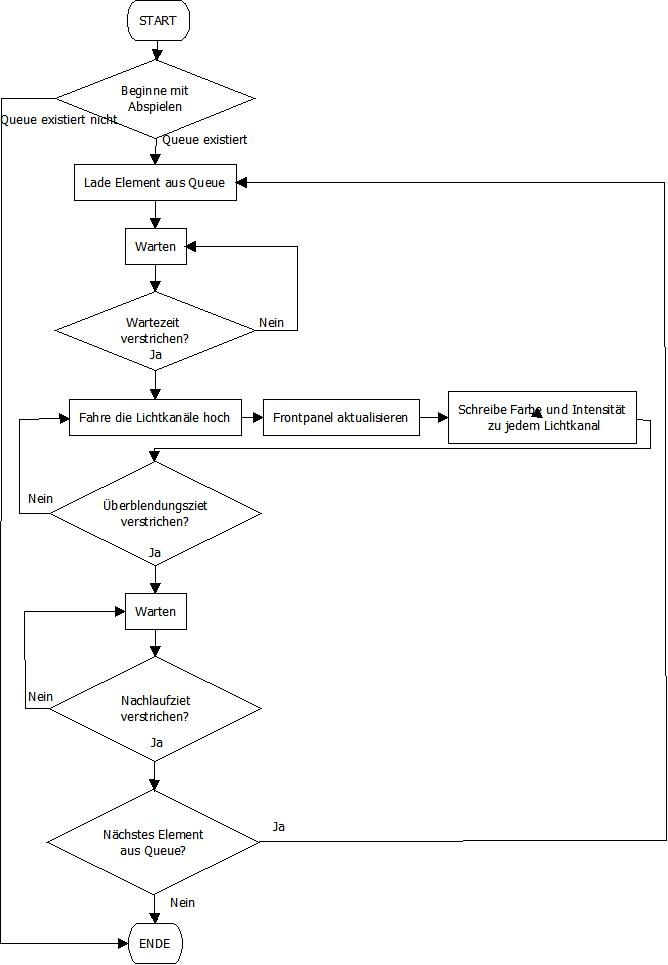
\includegraphics[height=0.72\textheight]{Pics/play-flowchart.jpeg}
	\caption{Ablaufdiagramm für die Abspiel-Funktion}
	\label{fig:plan01}
	\end{figure}	
		
\subsection{Datenfluss Diagramm}
Datenfluss Diagramme haben die Aufgabe zu zeigen, welchen Weg die Daten durch eine Applikation nehmen. Abbildung \ref{fig:plan02} zeigt das Datenfluss Diagramm für die Abspiel-Funktion in der Party-Licht-Steuerung. Die Knoten (Kreise) repräsentieren die Prozesse. Eine externe Entität ist das Licht Kontroll-System.  Die Pfeile zeigen den Datenfluss.
	\begin{figure}[h!]
	\centering
		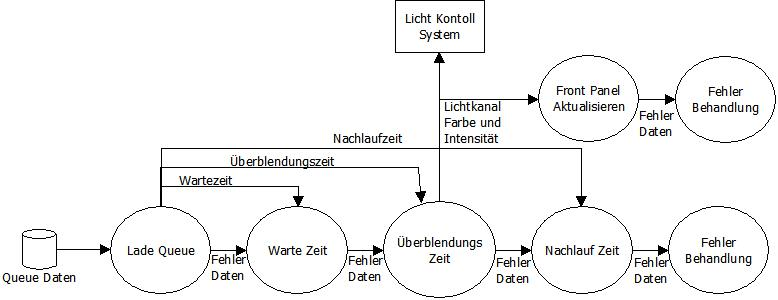
\includegraphics[width=\textwidth]{Pics/play-dataflow.jpeg}
	\caption{Datenfluss Diagramm für die Abspiel-Funktion}
	\label{fig:plan02}
	\end{figure}	
		
\section{User Interface}

\section{Code Implementierung}
		\subsection{Auswahl des Design Pattern} %6-3
		%4-18
		\subsection{Timing}
		\subsection{Auswahl der Datentypen}

		\subsection{Init und Shutdown Funktion}	%E 7-1
		\subsection{Aufnahme-Funktion}	
		\subsection{Abspiel-Funktion}
		\subsection{Stopp-Funktion}
		\subsection{Speichern und Lade Funktion}
			
		\subsection{Fehlerbehandlung}

\section{Testen}		

\section{Anwendung}
	\subsection{Stand-Alone Applikation}
	\subsection{Installer}
	\subsection{Webservice}

\section{Abschließende Betrachtung}
	\subsection{Update }%E8-2
	\subsection{Information Hiding} %E4-5
	\subsection{Erweiterungen}
	Hardware Ansteuerung, Visualisierung größer

